\section{Logistic Regression}

Logistic regression fits an S-shaped \textit{logistic function} to model binary outcomes (e.g., true/false). Linear regression, by contrast, fits a straight line to a continuous target.

In binary classification, the logistic curve ranges from 0 to 1. It reads on the y-axis as the probability of an event, given a predictor value on the x-axis, so higher x-values map to higher probabilities.

\begin{wrapfigure}{r}{0.3\textwidth}
\centering
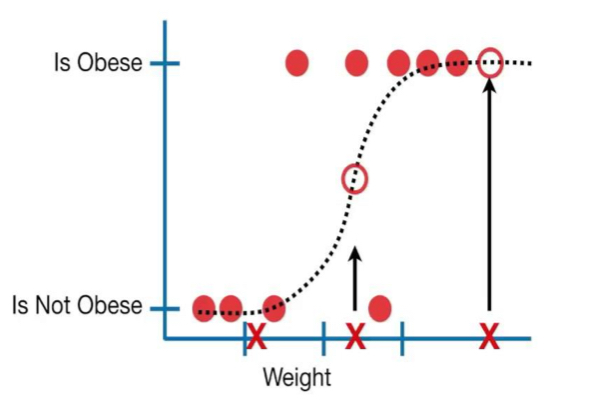
\includegraphics[width=\linewidth]{img/IMG_2215.jpeg}
\end{wrapfigure}

\paragraph{Key Difference: Linear vs Logistic Regression}
Linear regression minimizes the sum of squared residuals through the least squares method. Logistic regression has no residuals to minimize, so it fits its curve by \textbf{Maximum Likelihood Estimation (MLE)}. The steps are:

\begin{itemize}
    \item Assign a probability to each observation based on the model.
    \item Calculate the likelihood of each observed outcome.
    \item Multiply all likelihoods to get the total likelihood.
    \item Adjust the curve and repeat.
    \item Select the curve that maximizes the overall likelihood.
\end{itemize}

\begin{figure}[h]
    \centering
    \begin{subfigure}[b]{0.22\textwidth}
        \centering
        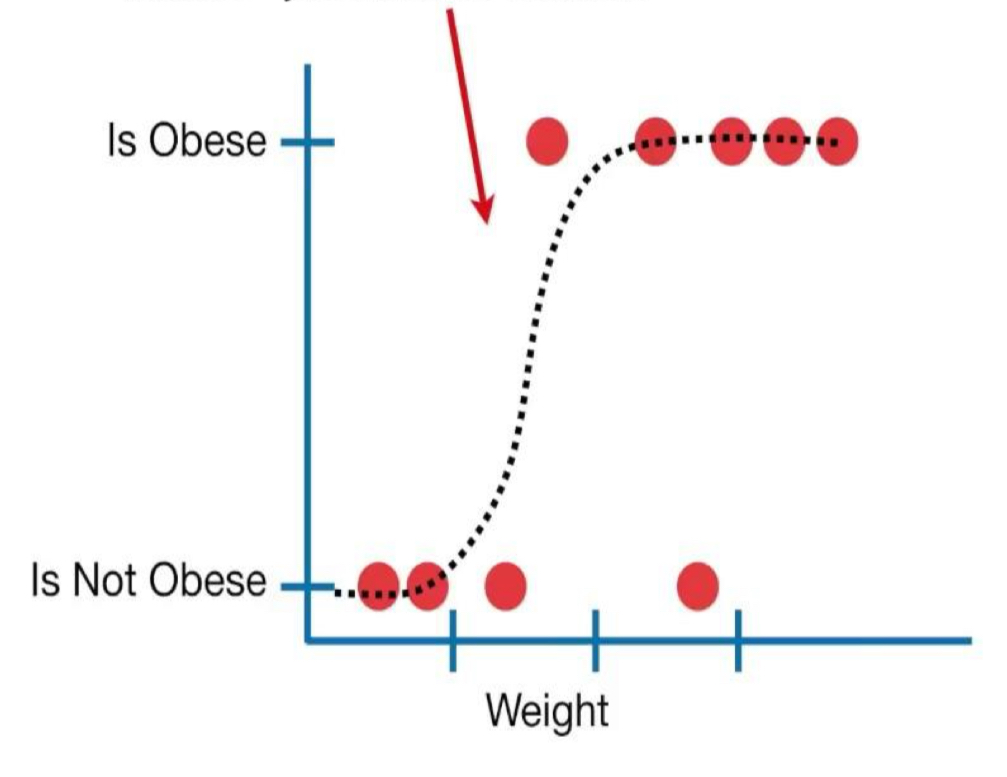
\includegraphics[width=\textwidth]{img/IMG_2221.jpeg}
        \caption{Assign a probability.}
    \end{subfigure}
    \hfill
    \begin{subfigure}[b]{0.22\textwidth}
        \centering
        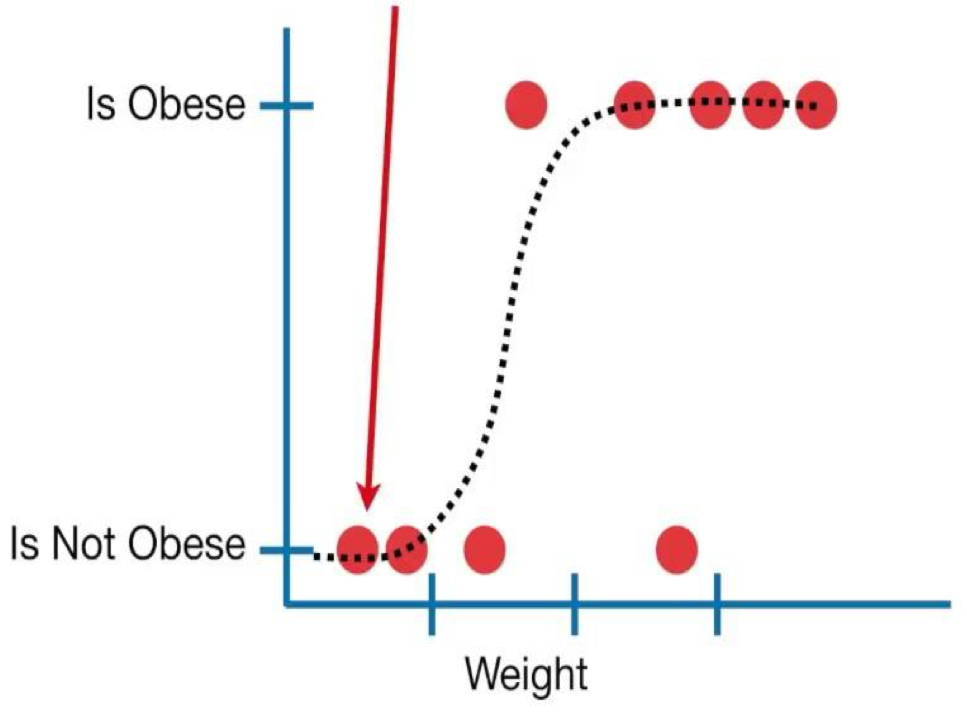
\includegraphics[width=\textwidth]{img/IMG_2222.jpeg}
        \caption{Compute likelihood.}
    \end{subfigure}
    \hfill
    \begin{subfigure}[b]{0.22\textwidth}
        \centering
        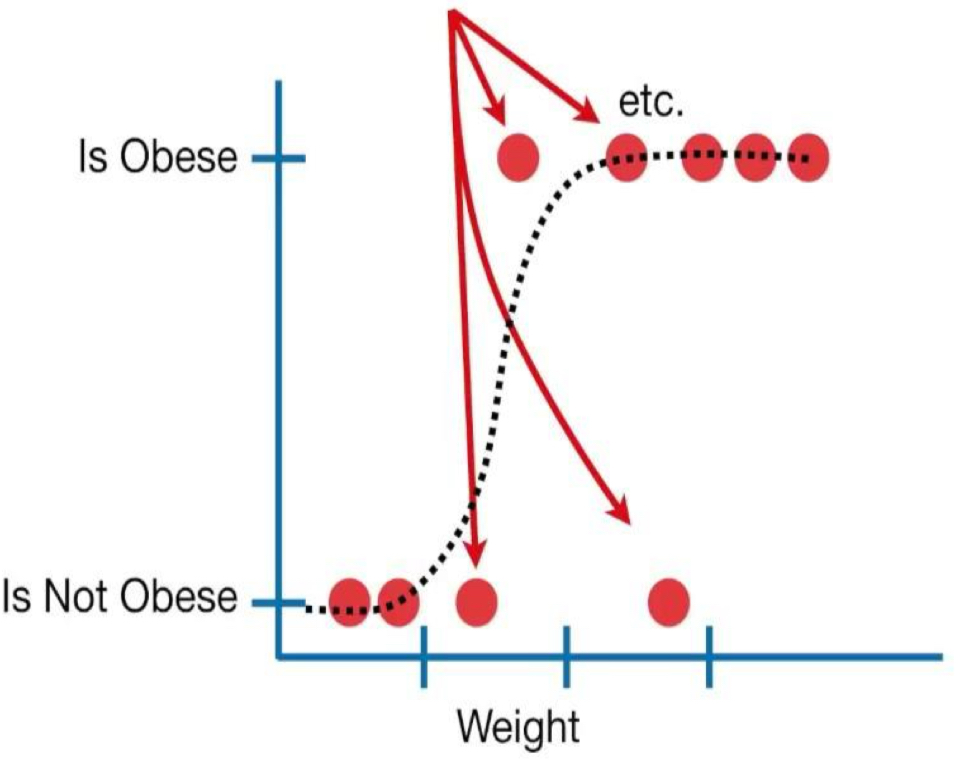
\includegraphics[width=\textwidth]{img/IMG_2223.jpeg}
        \caption{Repeat for each point.}
    \end{subfigure}
    \hfill
    \begin{subfigure}[b]{0.22\textwidth}
        \centering
        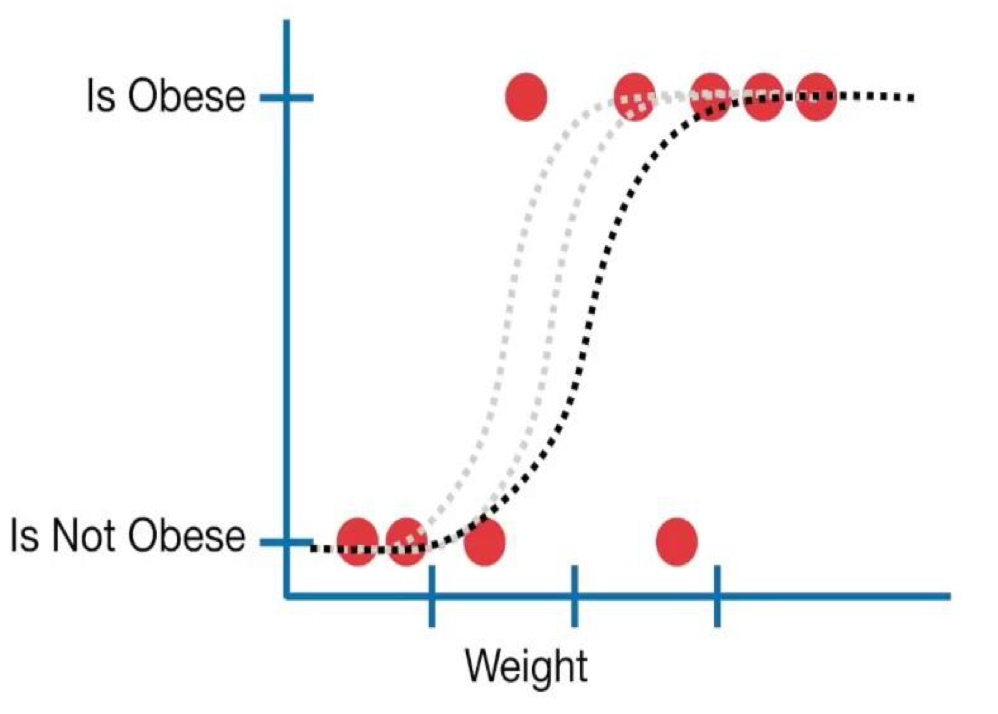
\includegraphics[width=\textwidth]{img/IMG_2224.jpeg}
        \caption{Adjust the line.}
    \end{subfigure}
    \caption{Steps in Maximum Likelihood Estimation.}
\end{figure}

\subsection{Logistic Regression and the Logit Function}

\begin{wrapfigure}{r}{0.2\textwidth}
\centering
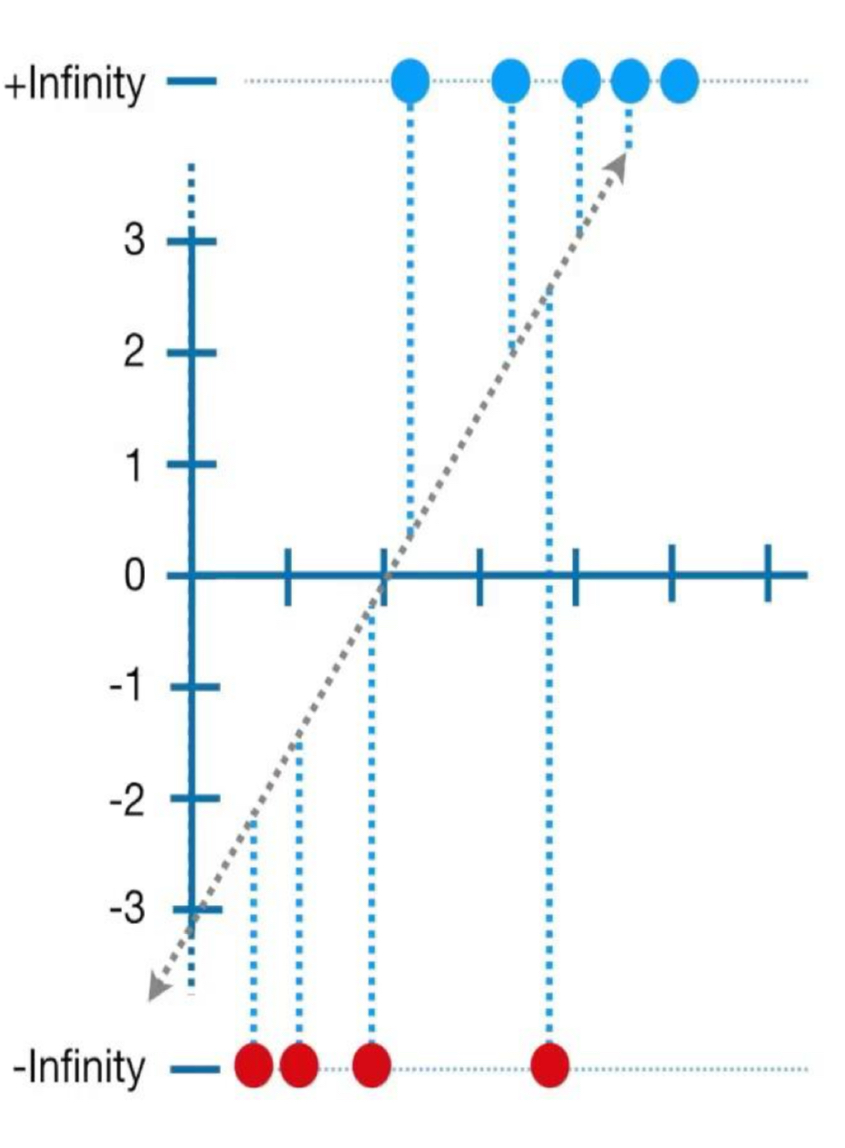
\includegraphics[width=\linewidth]{img/IMG_2225.jpeg}
\end{wrapfigure}

Logistic regression models the log of the odds (logit) as a linear function of the input variable \(X\):

\[
\log\left(\frac{p}{1-p}\right) = \beta_0 + \beta_1 X
\]

We fit the candidate line in the transformed space (log-odds), then project it back into probability space:

\begin{equation}
p = \frac{e^{\text{log(odds)}}}{1 + e^{\text{log(odds)}}}
\end{equation}

\begin{figure}[H]
    \centering
    \begin{subfigure}[b]{0.45\textwidth}
        \centering
        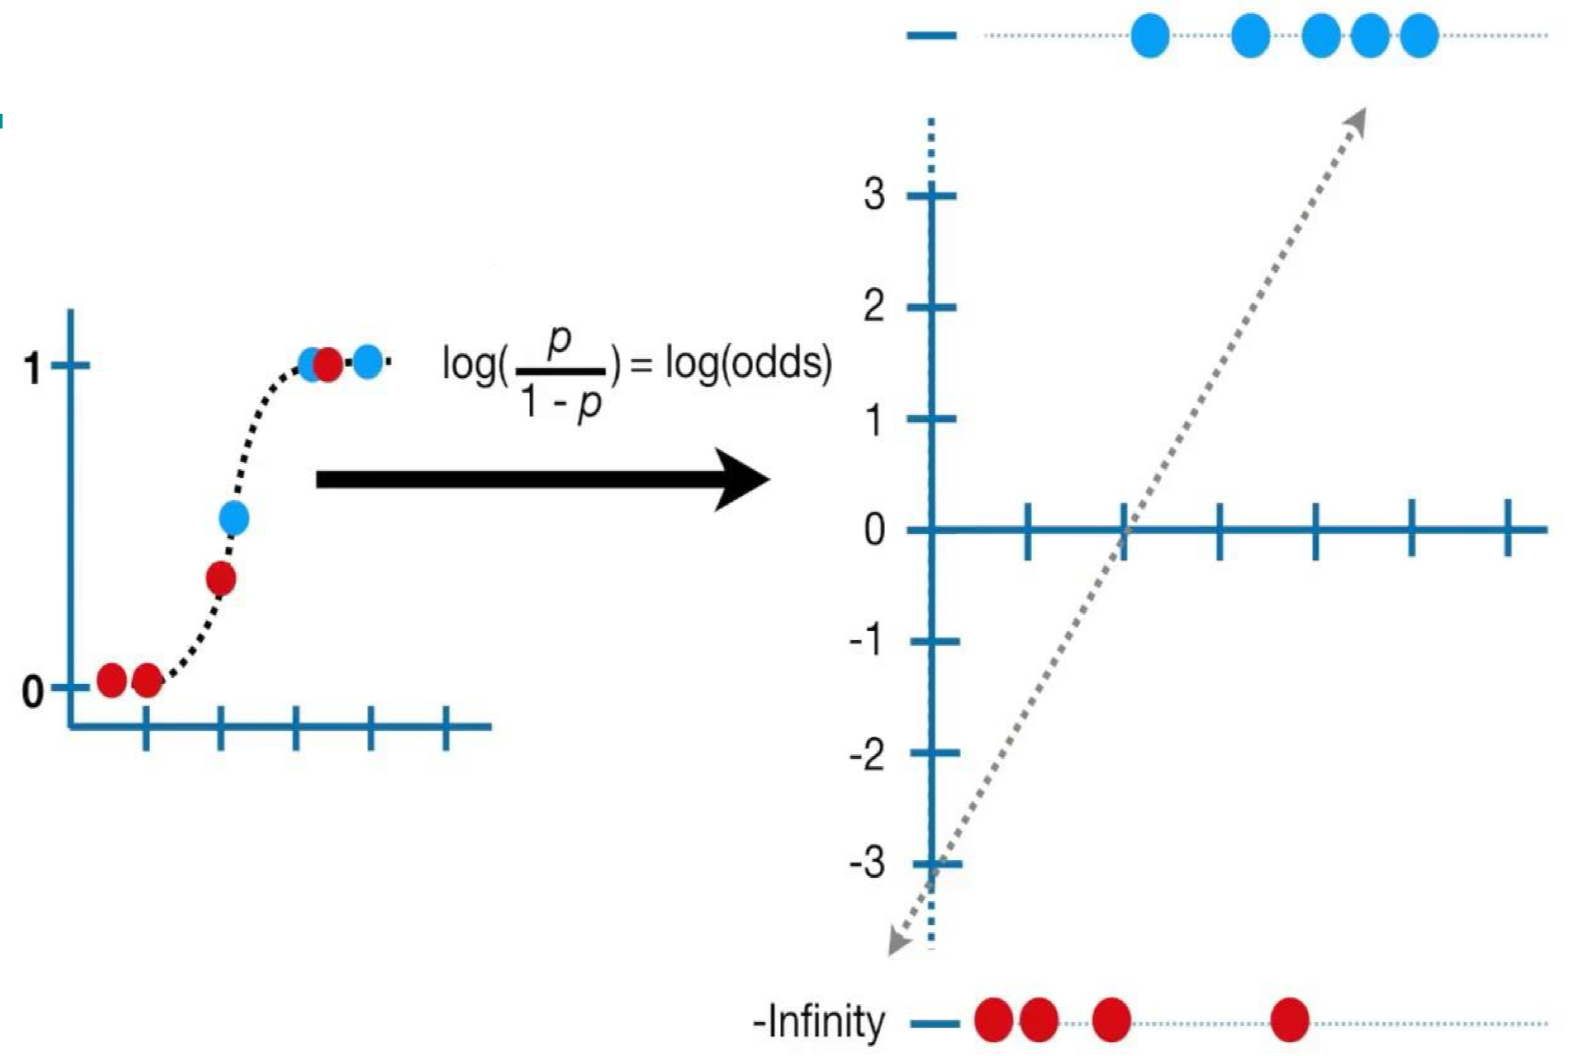
\includegraphics[width=0.6\textwidth]{img/IMG_2226.jpeg}
    \end{subfigure}
    \begin{subfigure}[b]{0.45\textwidth}
        \centering
        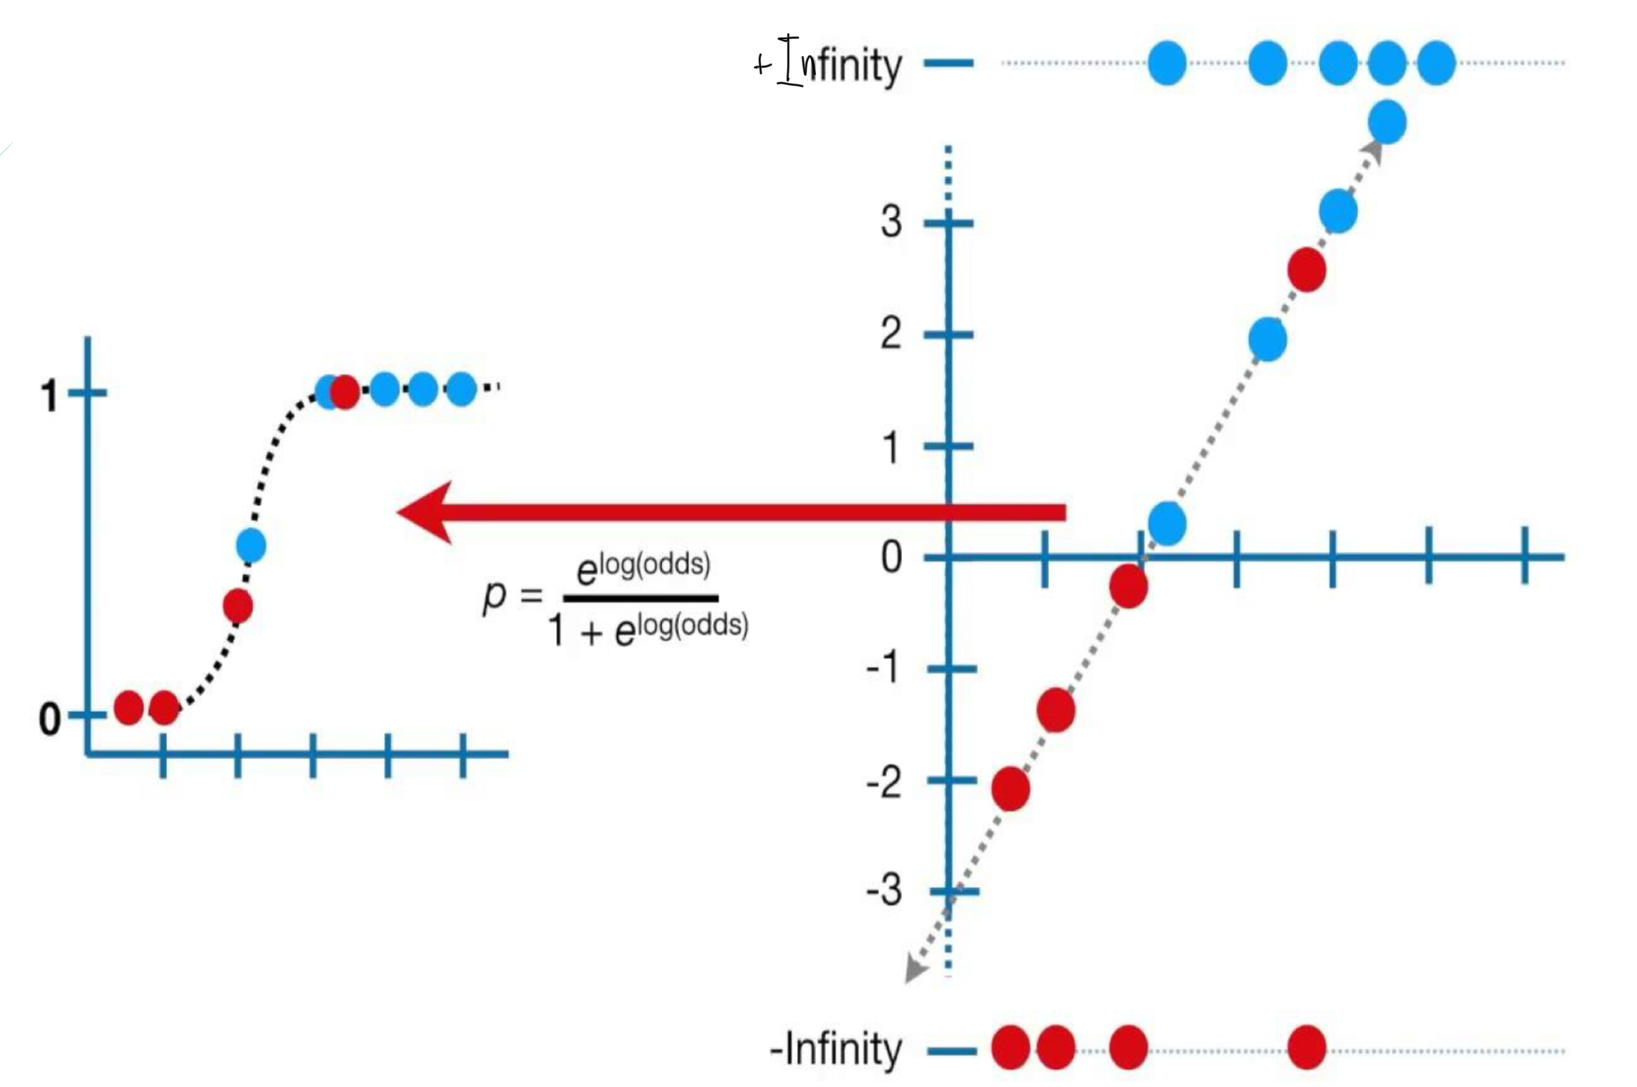
\includegraphics[width=0.6\textwidth]{img/IMG_2227.jpeg}
    \end{subfigure}
\end{figure}

This transformation is derived as follows:

\begin{align*}
\log\left(\frac{p}{1-p}\right) &= \text{log(odds)} \\
\Rightarrow \frac{p}{1-p} &= e^{\text{log(odds)}} \\
\Rightarrow p &= \frac{e^{\text{log(odds)}}}{1 + e^{\text{log(odds)}}}
\end{align*}

\subsection{Calculating the Likelihood}

Each data point is projected onto the candidate curve to yield a predicted probability, and that value is the likelihood of the observation. Since probabilities range from 0 to 1, multiplying many of them together drives the total likelihood toward zero. We therefore work with the \textbf{log-likelihood}, summing the logarithms of the individual likelihoods.

The fitting algorithm then:

\begin{itemize}
    \item Rotates and adjusts the candidate line,
    \item Recomputes the log-likelihood,
    \item Selects the line that maximizes the log-likelihood.
\end{itemize}

\textit{Result:} The optimal line is the one that maximizes the likelihood of observing the data under the model.

\subsection{Recovering Probabilities from Log-Odds}

\[
\ln\left(\frac{p}{1-p}\right) = \beta_0 + \beta_1 X
\quad \Leftrightarrow \quad
p = \frac{1}{1 + e^{-(\beta_0 + \beta_1 X)}}
\]

This is the \textbf{sigmoid function}, which maps any real-valued input to a probability between 0 and 1. Logistic regression thus models:

\begin{equation}
\text{logit}(p) = \log\left(\frac{p}{1-p}\right) = \beta_0 + \beta_1 X
\end{equation}

\textit{Interpretation:} The log-odds are linearly related to the predictor \(X\), enabling us to apply linear regression techniques in this transformed space.

\paragraph{Interpretation of \(\beta_1\)}

Let:
\[
\text{odds}_1 = \frac{p}{1-p} \quad \text{at } X, \quad
\text{odds}_2 = \frac{p}{1-p} \quad \text{at } X+1
\]

Then:

\begin{equation}
\frac{\text{odds}_2}{\text{odds}_1} = \frac{e^{\beta_0 + \beta_1(X+1)}}{e^{\beta_0 + \beta_1 X}} = e^{\beta_1}
\end{equation}

Thus \(e^{\beta_1}\) is the multiplicative change in odds for each one-unit increase in \(X\). The further this odds ratio sits from 1, the stronger the effect of \(X\) on the outcome \(Y\).